\documentclass[conference]{IEEEtran}
\IEEEoverridecommandlockouts
% The preceding line is only needed to identify funding in the first footnote. If that is unneeded, please comment it out.
%MMM\usepackage{cite}
\usepackage{amsmath,amssymb,amsfonts}
\usepackage{algorithmic}
\usepackage{graphicx}
\usepackage{textcomp}
\usepackage{xcolor}
\def\BibTeX{{\rm B\kern-.05em{\sc i\kern-.025em b}\kern-.08em
    T\kern-.1667em\lower.7ex\hbox{E}\kern-.125emX}}
    
    %MMM
\usepackage[
    natbib=true,
    style=numeric,
    sorting=none
]{biblatex}
\usepackage[english]{babel}
\usepackage{minted}
\usepackage{fancyvrb}
\usepackage{listings}    
    %mmm
\lstdefinelanguage{JavaScript}{
  keywords={typeof, new, true, false, catch, function, return, null, catch, switch, var, if, in, while, do, else, case, break},
  keywordstyle=\color{blue}\bfseries,
  ndkeywords={class, export, boolean, throw, implements, import, this},
  ndkeywordstyle=\color{darkgray}\bfseries,
  identifierstyle=\color{black},
  sensitive=false,
  comment=[l]{//},
  morecomment=[s]{/*}{*/},
  commentstyle=\color{purple}\ttfamily,
  stringstyle=\color{red}\ttfamily,
  morestring=[b]',
  morestring=[b]"
}

\lstset{
   language=JavaScript,
   backgroundcolor=\color{white},
   extendedchars=true,
   basicstyle=\footnotesize\ttfamily,
   showstringspaces=false,
   showspaces=false,
   numbers=left,
   numberstyle=\footnotesize,
   numbersep=9pt,
   tabsize=2,
   breaklines=true,
   showtabs=false,
   captionpos=b,
   xleftmargin=.25in,
   xrightmargin=.25in
}
    
    
\bibliography{template.bib}

\usepackage{comment}
 
    
    
    
    
\begin{document}




\title{Synchronization of Web Application with Broadcast
TV\\}
 

\author{\IEEEauthorblockN{Kafil Hussain}
\IEEEauthorblockA{\textit{TU Berlin} \\
\textit{Fraunhofer-FOKUS-Institut  }\\
Berlin, Germany \\
Email: kafil.hussain@campus.tu-berlin.de}



\and
\IEEEauthorblockN{Mohamed Mesto}
\IEEEauthorblockA{\textit{TU Berlin} \\
\textit{Fraunhofer-FOKUS-Institut  }\\
Berlin, Germany \\
m.mesto@campus.tu-berlin.de }\hfill \break


\and

\IEEEauthorblockN{Mustafa Darkshly}
\IEEEauthorblockA{\textit{TU Berlin} \\
\textit{Fraunhofer-FOKUS-Institut  }\\
Berlin, Germany \\
Email: m.darkshly@campus.tu-berlin.de}





\and

\IEEEauthorblockN{Malik Haroon Akbar}
\IEEEauthorblockA{\textit{TU Berlin} \\
\textit{Fraunhofer-FOKUS-Institut  }\\
Berlin, Germany \\
Email: m.akbar@campus.tu-berlin.de}
}

\maketitle

\begin{abstract}
HbbTV ( Hybrid broadcast broadband TV) is the
standard for the broadcast and broadband services, which also
provides customers to interact with their TV. The latest version of
HbbTV 2.0, which was released in 2015. This latest release added
some new features like HTML5, compatibility of companion
screens and multi device synchronization. In our project well
be using MPAT as HbbTV development environment. Which is
basically a WordPress based applications and provides easy to
use development environment for even programing beginners. In
this project well be developing an MPAT based plugin, that will
allow viewers of ”Jede Antwort zhlt!” to play quiz along the TV
show. As the theme of quiz show is to present multiple choice
questions. TV viewers will be able to select correct answers, and
their scores will be shown on screen. Which will make show more
interesting for show audience at home. And behind the scenes,
there will be another actor (editor), who will interact with this
application. An admin panel will be show on the editor side, who
will be able to enter the numbers of questions, time stamps and
score for each question. This plugin will provide synchronisation
in such a way that it will only show components on screen when
there will be questions on screen.




\begin{IEEEkeywords}
component, formatting, style, styling, insert

\end{IEEEkeywords}
\end{abstract}


 

\section{\textbf{Introduction}}\label{sec:Introduction}
Hybrid broadcast broadband TV (or HbbTV) is a global
initiative aimed at harmonizing the broadcast and broadband
delivery of entertainment services to consumers through
connected TVs, set-top boxes and multiscreen devices. The
HbbTV specification is developed by industry leaders to improve
the video user experience for consumers by enabling innovative,
interactive services over networks. The specification
uses elements of existing specifications from other standards
including OIPF, CEA, DVB, MPEG-DASH and W3C. With
the incorporation of activities from the Open IPTV Forum
(OIPF) in 2014 and Smart TV Alliance in 2016, HbbTV is able
to address service providers and technology suppliers for IPTV
services as well as the combined scope of broadcast and overthetop services \footnote{https://www.hbbtv.org/news-events/hbbtv-releases-version-2018-2-of-the-hbbtv-conformance-test-suite//}. Jede Antwort zhlt is the famous german
game show, theme of the show is to present questions and
for each correct answer participants get cash prizes. There are many other games show on same theme and mostly they catch
their audience attention with the valuable information they
provide in questions. And they make it more interesting by
awarding money on each answer\cite{hbbtv}. RBB-Quiz Plugins objective
is to make Jede Antwort zhlt more interesting for audience
watching game show at home. Quiz plugin will allow viewers
to interact with this TV, and they well be able to play quiz
along with the game show. This interactive experience will
catch more engagement of home audience, and show will
become more interesting for them as they will feel like they are
actually in the show and playing. MPAT takes up the concept
of web-page creation tools like WordPress, which allow users
to easily build a small to medium web site from pre-defined
templates and plug-ins, and adapts it to HbbTV  \footnote{https://github.com/MPAT-eu/MPAT-theme/blob/master/getContent.php}. So, well
be using plugin feature of wordpress to interact with wordpress
and MPAT powers. Firstly, this plugin will show the video of
quiz show on viewers Hbbtv screen, and when then host will
ask question on show, our plugin will also trigger an event
to show some components on screen. User wills interact with
these components by using his remote and he/she will submit
answer\cite{MPAT}. If the answer will be right, then user will get score
which will be update on the screen after the host will reveal
answer in the show. Secondly, before the broadcast of tv show
an editor will also interact with the admin panel of quiz plugin,
where he/she will be able to configure questions, answers,
time stamps and worth of question. Events on the viewer side
will be triggered on screen, by using all these details provided
by editor on admin panel by the editor.
\section{\textbf{RELATED WORK}}\label{sec:RELATED WORK}

A predecessor of MPAT, named HAT (developed in the FICONTENT
2 project) has already been used to provide a childfriendly
sub-site for a German public broadcaster. The HbbTV
Application Toolkit (HAT) is an easy and cost-efficient way
for content creators to produce HbbTV applications. It is based
on the WordPress concept of providing tested templates and
components so content creators have an easy migration path.
For producing TV content, HAT only requires the same skill
set as for web page creation. Due to the separation of layout
templates and content, content creators can focus on their
content on screen without worrying about styles or maintaining
the required corporate design. These are already optimized for
TV use and ensure that an application created with HAT will
follow established rules for TV application development and
usage [3].
















 Figure \ref{fig:Use-case-Diagram}.

\begin{figure}[!ht]
	\centering
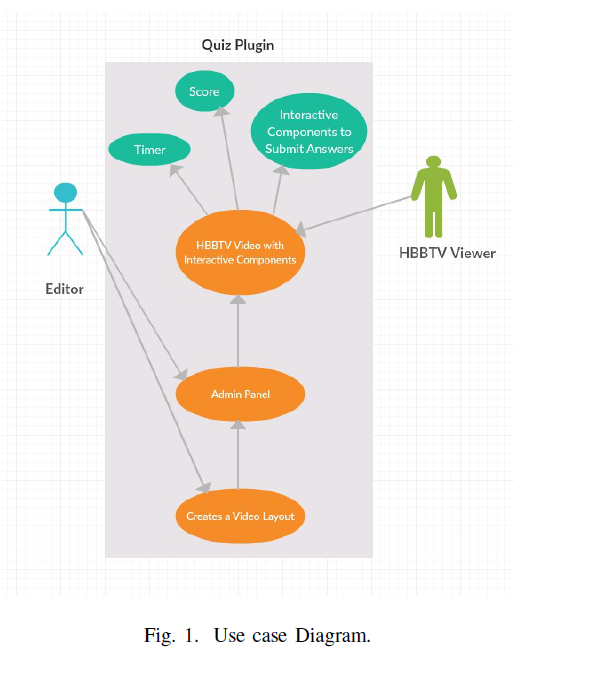
\includegraphics[scale=0.6]{figures/Use-case-Diagram.png}\\
	\caption{Use case Diagram }
	\label{fig:Use-case-Diagram}
\end{figure}
 

 
    
\section{\textbf{Setting up the development environment }}\label{sec:relatedwork}

\subsection{Dynamic ad-insertion and content orchestration workflows through manifest manipulation in HLS and MPEG-DASH}

The work presented in \cite{adinsertion} uses Manifest manipulation to dynamically insert ads into media content with the FAMIUM DAI solution. This study mentions how HLS specifies a so-called \#EXT-X-DISCONTINUITY tag, which is used in the manifest file to decorate a generic discontinuity at the source. This could be a switch of e.g. encoding parameters, input sources, or an advertisement, which has been spliced into the source. This was useful in our work to concatenate segments from different video sources, which will be explained in more detail in the Our approach section

This work has a component named The Manifest Stitcher, which performs individual manifest stitching, based on content playlists served by another entity in their architecture. The component creates MPEG-DASH and HLS manifests on the fly. The Stitcher requests the manifest files for the original content assets as well as for the pre-conditioned ad asset and creates a new manifest comprising multiple periods. This new manifest is sent to the client and allows him to play the individual stitched content.

The basic idea behind that approach is to ingest content or ads into DASH and HLS Streams by repackaging the stream. The output stream behaves like a linear stream, just like our use case for a single stream containing multiple input video streams. The re-packaged content can be handled by the player in the same way as the linear original stream. To guarantee smooth playback without re-initialization of the video player, it is necessary to condition the original stream and the content to be inserted with the same content specifications in terms of audio and video coding settings. These last conditions are also considered for our work, streams with different audio formats will not play properly.
 
\subsection{ABR streaming with separate audio and video tracks: measurements and best practices}

This paper \cite{measures} examines the state of the art in the handling of demuxed audio and video tracks in predominant Adaptive Bitrate Streaming protocols (DASH and HLS). They found several limitations in existing practices both in the protocols and the player implementations, which can cause undesirable behaviors such as stalls, selection of potentially undesirable combinations such as very low-quality video with very high-quality audio, etc. Our work had to handle streams with separate audio tracks, having to join both video and audio segments in separate manifest files without consideration on how well is the quality of experience; this matter will be covered in the Evaluation and Results section.

\subsection{Increasing ad personalization with server-side ad insertion}

This paper \cite{ssai} examines the architectures required to achieve server-side advertisement insertion so that multiple concurrent advertising manifests can be delivered in a timely fashion. Cloud and cloud-assisted software solutions were required. 

When a video plays, the player makes the necessary calls to obtain the next chunk of content to be shown from the manifest. In a well-designed player, where the segments come from the same source, there should be a seamless display and a reasonable quality of experience. What is required, then, is a method of inserting targeted advertising into individual delivery paths that provides clear metrics, protects against advertising blocking or skipping, and maintains a consistent quality of experience for the consumer. The solution lies in upstream insertion of the advertising so that a continuous stream arrives at the consumer device eliminating any possibility of discrimination between content and commercials, and avoiding freezes, black screens, and spinning wheels.

In \cite{ssai}, is shown an HLS example manifest that uses the "\#EXT-X-CUE-OUT" manifest declaration, which is the signal to the player that this is a commercial break. When using client-side advertisement insertion, the player will have some sort of logic to initiate a call to get the advertisements. The player will probably download ads to play within the time between the CUE markers. During the "\#EXT-X-CUE" breaks, it is clear that some calls are not to the content provider but advertising servers. By moving the advertising insertion to the server side and within the packaging process, the content provider address and the advertisement server provider address differences are eliminated and made to look the same from a manifest perspective. There is no need to put the \#EXT-X-CUE tags anymore as the ad insertion or replacement is already done. The client's content and the ads would be hosted at the same address. 

This eliminates the prospect of skipping the advertising, a consistent stream of content is also presented in the same resolution, codec, and encryption, which maintains the quality of experience. Finally, a single contiguous stream is sent to the client.
\section{\textbf{Our Approach}}\label{sec:main}
\subsection{ Proposed Solution}

Based on the demand of the project we decided to use
Plug-in feature of WordPress since there were so many other
options like using the timeline feature of MPAT or developing
an application by using Multi-sites and a separate database.
etc. WordPress plugin is a piece of software written in PHP
that contains different functions and features to extend the
functionality of the WordPress environment, and it does not
change anything in the core functionality of WordPress. Plugins
functionality can be very elastic, and it can be simple like
just printing Hello World, or complex as plugins like Yoast
SEO for WP plugin.

\subsection{Technologies we used}
 We used the following technologies for developing out plugin
in order to complete the project.


\begin{enumerate}
  \item PHP: 
In the plugin development, the first skill you need is PHP
skills. There are some basic protocols one has to follow in the
plug-in like, the name of the plugin, plugin URI, Description
of the plugin, version of the plugin, Authors URI, name of the
authors and last the license. PHP functions and some hooks
for the attachment of functions, to maintain the functionality
of plugin or to attach different function together.
 \item avascript: 
A scripting language which is commonly used in client side.
It is used to provide for a more user-friendly experience such
as dynamically updating web pages.
In the context of our project, we used javascript for different
purposes such as, triggering different events like, buttons,
When to appear in the screen and which time of the video,
adding the score of the user, updating the score.
 \item CSS: 
CSS is the language that defines the design of HTML
documents. In our project, we used it for designing all the
components on video those will appear on the user side like
timing, score, and options to select answers. The color of the
buttons when they appear in the screen and the color will
change once the user selects the answer. On the admin panel,
the design of the input form.
 \item  HTML: 
A standard markup language, HTML (Hypertext Markup
Language), is used for developing the web pages and web
applications. In HTML we use different other languages like
CSS, Javascript for different purposes like the design, style of
the text, color and so many other features.
Currently HbbTv 2.0 is the latest version which supports
HTML5, and older versions HbbTV 1.0 and 1.5 supports
HTML 4. So, while the development of MPAT plugin, we
used HTML5.
\end{enumerate}


\subsection{Plugin Installation and Activation}


MPAT plugin Installation is the same as other simple
WordPress plugins. The only difference will be we need to
copy the plugin file in different folders. MPAT RBB-Quiz
plugin resides on the following paths.


\begin{enumerate}
\item Linux: /opt/lampp/htdocs/MPAT-coremaster/
web/app/plugins/mpat-plugins
\item Windows OS : C:/Xamp/htdocs/MPAT-coremaster/
web/app/plugins/mpat-plugins
\end{enumerate}

When plugin files are placed in the respective directories,
then they will show in plugin names (RBB-Quiz) in the plugin
list of WordPress. Then Well just need to click the activate
button to start its functionality. Following use case diagram
shows how administrator and TV viewer will interact with the
plugin.


When RBB-Quiz plugin is activated, in WordPress it creates
a page named as RBB-Quiz-Page, Which will be linked with
the layout created by admin manually, and administrator will
also be responsible for adding video source link in components
settings.



 






 Figure \ref{fig:Use-case-Diagram}.

\begin{figure}[!ht]
	\centering
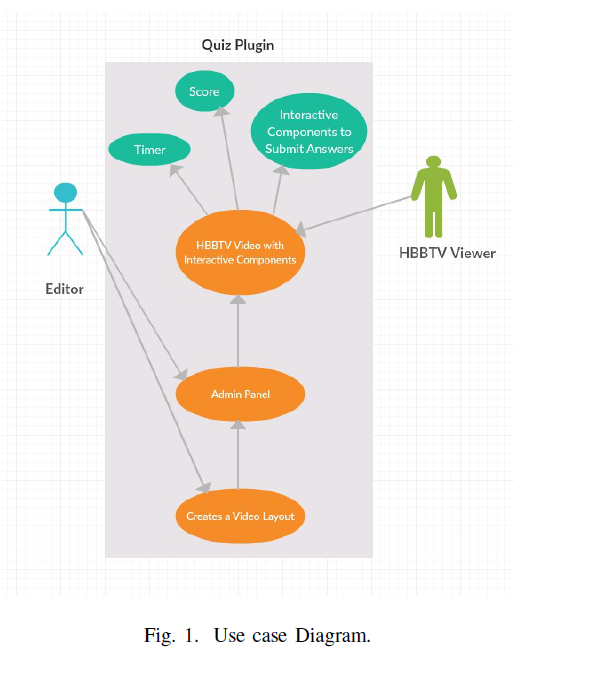
\includegraphics[scale=0.6]{figures/Use-case-Diagram.png}\\
	\caption{Use case Diagram }
	\label{fig:Use-case-Diagram}
\end{figure}
 
After that administrator’s responsibility will be to login to
admin panel and fill the details about questions. In the admin
panel, first of all, the admin will enter the question number,
which is just a sequence number of question in the database.
It has no effect on triggering events on screen. Secondly, the
admin will enter the start time of the question according to
the video, the end time of the question. These timestamps
will be responsible for triggering events on the screen such
as showing buttons to submit answers and these buttons will
disappear when question time expires. In the last section of this
form, the admin will enter the score for and correct answer for
that question. This information will verify the correct answer
to the question and updates the score accordingly.
 
    
   

 Figure \ref{fig:Admin-panel}.

\begin{figure}[!ht]
	\centering
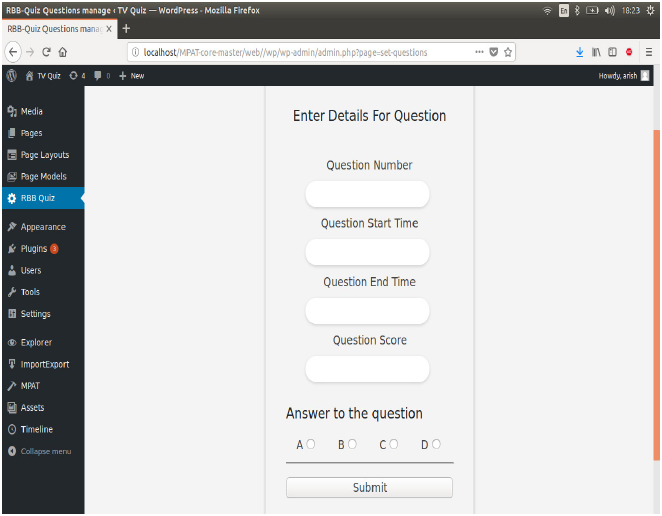
\includegraphics[scale=0.6]{figures/Admin-panel.png}\\
	\caption{Admin Panel}
	\label{fig:Admin-panel}
\end{figure} 
    
    
    
    
    
    
    
    
    
    
    

    
    
    

\subsection{TV User Interface}

When the video starts streaming, the HbbTV plugin will
populate the TV screen with different components. Following
are the components with their details: Figure \ref{fig:User-interface}.


    
    \begin{itemize}
       \item Timer Component
\item Score Component
\item Buttons to Submit Answer
    \end{itemize}




\begin{figure}[!ht]
	\centering
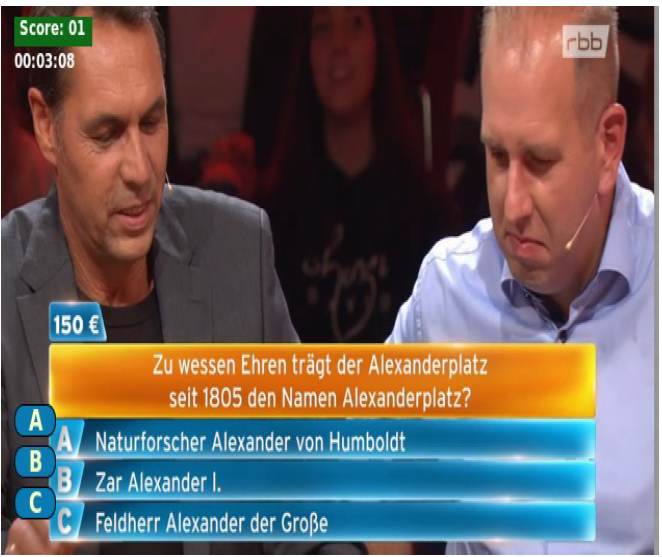
\includegraphics[scale=0.6]{figures/User-interface.png}\\
	\caption{User interface}
	\label{fig:User-interface}
\end{figure}




 \begin{enumerate}
 \item  Timer Component: 
 
 Timer component will show the current time on the video,
timer value will also be used to show answer components on
the score. When the time on time counter will be the same as
the time mentioned as the start time of question. Then exactly
on that time new components will appear on screen, where the
user can make the decision and selects the answer by the given
time for the question by the administrator of the show. For
each question, there is a start time and end time. In between
that time user has to make the decision and select any of the
possible answers.
 \item  Score Component: 
 
 Score component will always be there on the screen, but
it will update scores only when the video reaches at the end
time of each question. Total scores will be updated after every
question. The total core is dependent on the weights that the
administrator provides for each answer. The scoring algorithm
simply counts the weight of submitted answer and then adds
it to the current score value. If the user does not select any
answer the score will be zero. Once the user selects the answer
it will be locked and the right answer will appear after the
expiry of question time.
 \item  Buttons to Submit Answer:
 
 When TV host will announce the question in the Jede
Antwort zhlt, on the users screen three clickable buttons will
appear and these buttons will stay on screen until the question
time expires. User will only be able to select the answer only
once, and it will be locked until the right answer will be
revealed in the show. When the answer will be revealed the
player’s score will be updated in the core component.
Once the user selects the answer the color of the selected
answer will be changed and its locked. User will not be able
to change the answer once it is selected.
\end{enumerate}

 
\section{\textbf{Results and Discussion}}\label{sec:Evaluation} 

To test the Master Manifests, Safari Web Browser was used as it has native HLS support in its video player. The VLC video player was an option but it produced playback errors when switching streams, the player restarted the counter instead of having continuity. Native HLS Playback Google Chrome extension was also tested, but it produced playback errors between streams. Safari had the best performance for testing. The idea is to have the streams mixed into a single stream playing sequentially.

Because we are writing the master manifest in a local file on our computer, we need a localhost server running so the videos can be played in Safari. We used the following python command in the Unix environment:  \Verb|python3 -m http.server|
To play the stream in the Safari search bar, one types \textcolor{blue}{http://localhost:8000/master.m3u8}

We also have a Node JS testing application which will serve us as our external application and imports the video mixer library as a dependency. This application has a main.js file that calls the \Verb|algorithmA()| and \Verb|algorithmB()| methods.

\subsection{Strategy 1}

We tested the first strategy, which consists of having as an output a final manifest that will have the representations present only for the first element of the input array. In this case, we made an HLS file which is hosted in our computer for testing purposes. The Node JS application calls the first strategy method with three input streams:

\begin{lstlisting}
algorithmA(["http://localhost:8000/puskasStream/master.m3u8",
    "https://playertest.longtailvideo.com/adaptive/oceans_aes/oceans_aes.m3u8",
    "https://test-streams.mux.dev/pts_shift/master.m3u8"])
\end{lstlisting}

The three streams have respectively these resolutions: 

\begin{itemize}
\item 1280x720
\item 304x128, 384x160, 544x224, 736x304, 960x400, 1264x528
\item 480x270, 768x432, 864x486, 1280x720
\end{itemize}

Once the localhost server was running, we tested the first strategy. The first URL's resolution, which is the needed resolution, is 1280x720 and it is not present in the second stream but it is in the third one. Our final manifest as an output from the algorithm will have only one variant which is 1280x720 and makes a reference to the media playlist file that was created for this representation. The playlist file has all the segments from the two streams concatenated in a single list.

Here is the resulting Master Manifest which has the only resolution present in the first input stream, 1280x720. This variant has a media playlist and it does not include an audio track because the video segments have them integrated.

\begin{lstlisting}
#EXTM3U
#EXT-X-STREAM-INF:BANDWIDTH=2320000,
RESOLUTION=1280x720
1280x720.m3u8
\end{lstlisting}

Here is the media playlist manifest (simplified) for the 1280x720 resolution. This playlist has all the video segments from the two streams concatenated in a single list. In between the two streams, the \#EXT-X-DISCONTINUITY tag has to be inserted.

\begin{lstlisting}
#EXTM3U
#EXT-X-VERSION:3
#EXT-X-TARGETDURATION:16
#EXT-X-DISCONTINUITY
#EXTINF:11.533333,
http://localhost:8000/puskasStream/All Puskas Award Winners (2009-2021)0.ts
#EXTINF:8.5,
http://localhost:8000/puskasStream/All Puskas Award Winners (2009-2021)1.ts
...
#EXT-X-DISCONTINUITY
#EXTINF:4.736,
https://test-streams.mux.dev/pts_shift/media-uoj0it22v_0.ts
#EXTINF:4.8,
https://test-streams.mux.dev/pts_shift/media-uoj0it22v_1.ts
...
\end{lstlisting}

\subsection{Strategy 2}

We tested the second strategy, which consists of the intersection of resolutions from the input URLs. The Node JS application calls the second strategy method with two input streams: 

\begin{lstlisting}
algorithmB(["http://amssamples.streaming.mediaservices.windows.net/634cd01c-6822-4630-8444-8dd6279f94c6/CaminandesLlamaDrama4K.ism/manifest(format=m3u8-aapl)", 
    "http://amssamples.streaming.mediaservices.windows.net/91492735-c523-432b-ba01-faba6c2206a2/AzureMediaServicesPromo.ism/manifest(format=m3u8-aapl)"])
\end{lstlisting}

The two streams have respectively these resolutions: 

\begin{itemize}
\item 640x360, 960x540, 1280x720, 1920x1080, 2560x1440, 3840x2160, 4096x2304
\item 320x180, 640x360, 960x540, 1280x720, 1920x1080
\end{itemize}

The intersection of all resolutions is: 640x360, 960x540, 1280x720 and 1920x1080

For simplicity, we are going to call Stream1 and Stream2 to replace the URLs in the video segments addresses, also, we are not listing the complete playlist.

We can see that for these three streams we have four representations resulting from the intersection. The representations 640p, 960p, 1280p, and 1920p are present in these three streams. We have as output files four representations along with the master manifest. We can see that our master manifest has now four variants, each of them referring to the media playlist file which has the name of the resolution. We have all the segments or clips concatenated for the three streams.

Here is the resulting Master Manifest from the intersection of the resolutions from the input streams. Four variants are present, each with its m3u8 playlist manifest. The two matching streams each had audio tracks themselves, so each variant refers to the audio track.

\begin{lstlisting}
#EXTM3U
#EXT-X-MEDIA:TYPE=AUDIO,GROUP-ID="audio",
NAME="audio",URI="audio.m3u8"
#EXT-X-STREAM-INF:BANDWIDTH=1355199,
RESOLUTION=640x360,AUDIO="audio"
640x360.m3u8
#EXT-X-STREAM-INF:BANDWIDTH=2532741,
RESOLUTION=960x540,AUDIO="audio"
960x540.m3u8
#EXT-X-STREAM-INF:BANDWIDTH=2532741,
RESOLUTION=1280x720,AUDIO="audio"
1280x720.m3u8
#EXT-X-STREAM-INF:BANDWIDTH=2532741,
RESOLUTION=1920x1080,AUDIO="audio"
1920x1080.m3u8
\end{lstlisting}

Here is the audio playlist manifest (simplified). This playlist has all the audio segments from the two streams concatenated in a single list. In between the two streams, the \#EXT-X-DISCONTINUITY tag has to be inserted.

\begin{lstlisting}
#EXTM3U
#EXT-X-VERSION:4
#EXT-X-TARGETDURATION:11
#EXT-X-DISCONTINUITY
#EXTINF:10.026667
Stream1/QualityLevels(384000)/Fragments(aac_UND_6_384=100266666,format=m3u8-aapl)
#EXTINF:10.026667
Stream1/QualityLevels(384000)/Fragments(aac_UND_6_384=200533333,format=m3u8-aapl)
...
#EXT-X-DISCONTINUITY
#EXTINF:10.10068
Stream2/QualityLevels(53620)/Fragments(AAC_und_ch2_56kbps=101006802,format=m3u8-aapl)
#EXTINF:10.10068
Stream2/QualityLevels(53620)/Fragments(aac_UND_6_384=300800000,format=m3u8-aapl)
...
\end{lstlisting}

Here is the media playlist manifest (simplified) for the 640x360 resolution. This playlist has all the video segments from the two streams concatenated in a single list. In between the two streams, the \#EXT-X-DISCONTINUITY tag has to be inserted.

\begin{lstlisting}
#EXTM3U
#EXT-X-VERSION:4
#EXT-X-TARGETDURATION:11
#EXT-X-DISCONTINUITY
#EXTINF:10
Stream1/QualityLevels(926058)/Fragments(video=100000000,format=m3u8-aapl)
#EXTINF:10
Stream1/QualityLevels(926058)/Fragments(video=200000000,format=m3u8-aapl)
...
#EXT-X-DISCONTINUITY
#EXTINF:10.01
Stream2/QualityLevels(642832)/Fragments(video=100100000,format=m3u8-aapl)
#EXTINF:10.01
Stream2/QualityLevels(642832)/Fragments(video=200200000,format=m3u8-aapl)
..
\end{lstlisting}

\subsection{Discussion}

We can see that every time a playlist switches to a different content source (different stream), we add the \#EXT-X-DISCONTINUITY tag. The EXT-X-DISCONTINUITY tag indicates a discontinuity between the Media Segment that follows it and the one that preceded it. The EXT-X-DISCONTINUITY tag must be present if there is a change in file format or encoding parameters \cite{refs}. The client must be prepared to reset its parser and decoder before playing a Media Segment that has an EXT-X-DISCONTINUITY tag applied to it; otherwise, playback errors can occur. During the testing phase, when the tag was not present, the playback was failing when the player tried to switch to the next stream.
   
One use-case this project did not cover was mixing a stream that has audio tracks with one that doesn't. This would require, for future work, playing the audio playlist only in its correspondent video timestamp. It is assumed that timestamp manipulation is supported in HLS. Without timestamp manipulation, the stream that has audio integrated into each video segment plays with audio normally, when the player switches to the next stream, it has no audio because it depends on the audio tracks that were left out.

Additionally, if audio tracks are present in all matching streams, only one audio track is being included, for example, English audio. If other languages were available, the video mixer library would only choose the default audio.
\section{\textbf{Conclusions}}\label{sec:conclusions}

As a result of this project, users can enjoy, for example, a complete TV series in a single sit without interrupting the experience by refreshing the page for the next episode. Multiple streams can be played as a single one as long as they have matching resolutions and audio format.

This last feature is a future work that needs to be implemented and is considered a limitation in this present proof of concept as mentioned in the Discussion section, as well as multiple audio support where the user can choose, for example, which language audio to play.

Hls-parser was easy to work with and very intuitive. Some challenges were present when playlist URLs are in relative path format, so they had to be parsed and joined with the original stream address. In the initial stages of testing, video playback errors were present until further research discovered that the Discontinuity tag, mentioned in the Results section, was needed to have a smooth transition between streams.

The video mixer library leads to the beginning of a new era of streaming technologies, having as a goal to improve the user experience and, tentatively, to attach them to the web page for them to be exposed to more ads which leads to market profits.








%mmm\section*{References}

 





    %\bibliographystyle{IEEEtran} % enable for bibtex
    % enable for bibtex
    \printbibliography% enable for biber style
    % to show unreferenced publications ------------------------------------- */
    %\bibliographystyle{unsrt}
    %\cite{dummy}
    %\nocite{*}
    %------------------------------------------------------------------------ */

    % /* -------------------------------------------------------------------- */
    %\backmatter



\end{document}
